\section{Actividad No 03 – Consultas B\'asicas} 
		
\begin{enumerate}[1.]
	\item El departamento de Recursos Humanos requiere ampliar el reporte anterior (4.2.2) para hacerlo m\'as comprensible, por lo que se requiere que los encabezados de las columnas sean: Emp No, Empleado, Puesto y Fecha Contrataci\'on.
	\\
	\\SELECT emp.employee\_id AS 'Emp N', \\
	   emp.last\_name AS Empleado, \\
	   emp.job\_id AS Puesto, \\
	   emp.hire\_date AS 'Fecha de contrataci\'on' \\
	FROM employees AS emp; \\
	\begin{center}
	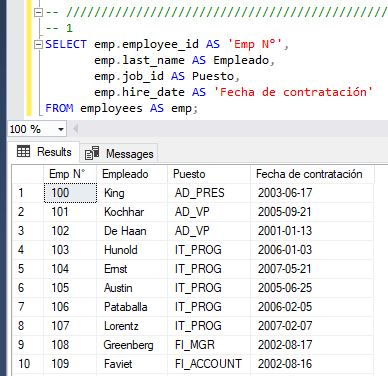
\includegraphics[width=5cm]{./Imagenes/actividad0301} 
	\end{center}

	\item Adicionalmente el departamento de Recursos Humanos requiere un reporte más sencillo, en el que se muestre los campos: last\_name y job\_id en una sola y \'unica columna (los datos deben estar separados por una coma) que tenga como alias Empleado y Puesto.
	\\
	\\SELECT CONCAT(emp.last\_name,',',emp.job\_id) AS 'Empleado y Puesto' \\
	\\FROM employees AS emp; \\
	\begin{center}
	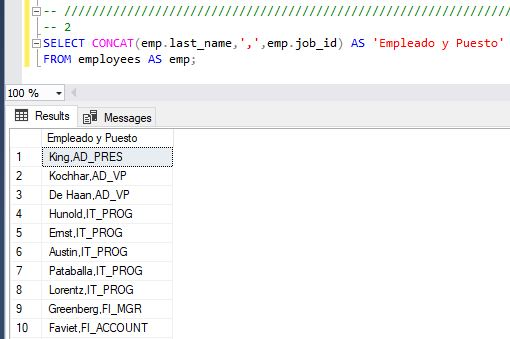
\includegraphics[width=5cm]{./Imagenes/actividad0302} 
	\end{center}

	\item Finalmente a modo de práctica, realizar una consulta que muestre todos los campos de la tabla EMPLOYEES, en una sola y única columna, los datos deben estar separados por una coma y la columna debe tener como encabezado Los Empleados
	\\
	\\SELECT CONCAT(emp.employee\_id,',', \\
			  emp.first\_name,',', \\
			  emp.last\_name,',', \\
			  emp.email,',', \\
			  emp.phone\_number,',', \\
			  emp.hire\_date,',', \\
			  emp.job\_id,',', \\
			  emp.salary,',', \\
			  emp.commission\_pct,',', \\
			  emp.manager\_id,',', \\
			  emp.department\_id) AS 'Los empleados' \\
	FROM employees AS emp; \\
	\begin{center}
	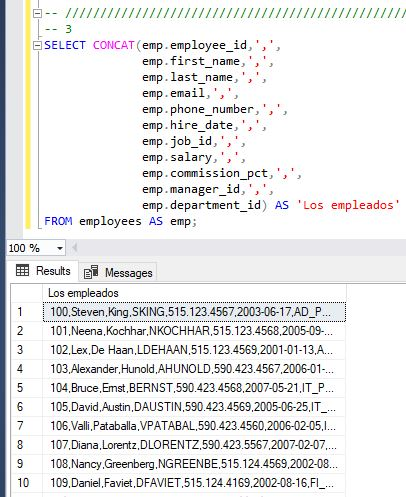
\includegraphics[width=5cm]{./Imagenes/actividad0303} 
	\end{center}

\end{enumerate}



